

\tikzset{every picture/.style={line width=0.75pt}} %set default line width to 0.75pt        

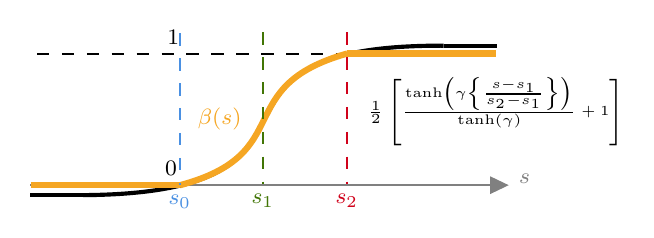
\begin{tikzpicture}[x=0.75pt,y=0.75pt,yscale=-1,xscale=1]
%uncomment if require: \path (0,215); %set diagram left start at 0, and has height of 215

%Straight Lines [id:da46631770507939163] 
\draw [color={rgb, 255:red, 128; green, 128; blue, 128 }  ,draw opacity=1 ]   (23,143.86) -- (250.5,143.86) ;
\draw [shift={(253.5,143.86)}, rotate = 180] [fill={rgb, 255:red, 128; green, 128; blue, 128 }  ,fill opacity=1 ][line width=0.08]  [draw opacity=0] (8.93,-4.29) -- (0,0) -- (8.93,4.29) -- cycle    ;
%Curve Lines [id:da39491275569940676] 
\draw [color={rgb, 255:red, 0; green, 0; blue, 0 }  ,draw opacity=1 ][line width=1.5]    (222.18,76.65) .. controls (87,76.16) and (185,147.66) .. (48.5,148.66) ;
%Straight Lines [id:da15611460318667292] 
\draw [color={rgb, 255:red, 0; green, 0; blue, 0 }  ,draw opacity=1 ][line width=1.5]    (23,148.66) -- (48.5,148.66) ;
%Straight Lines [id:da034171139038229326] 
\draw [color={rgb, 255:red, 0; green, 0; blue, 0 }  ,draw opacity=1 ][line width=1.5]    (222.18,76.65) -- (247.68,76.65) ;
%Straight Lines [id:da7075728897093001] 
\draw  [dash pattern={on 4.5pt off 4.5pt}]  (26.25,80.5) -- (247.25,80.5) ;
%Straight Lines [id:da5994500046428453] 
\draw [color={rgb, 255:red, 208; green, 2; blue, 27 }  ,draw opacity=1 ] [dash pattern={on 4.5pt off 4.5pt}]  (175.5,70.16) -- (175.5,143.41) ;
%Curve Lines [id:da28483688604328905] 
\draw [color={rgb, 255:red, 245; green, 166; blue, 35 }  ,draw opacity=1 ][line width=2.25]    (175.75,80.41) .. controls (119,96.41) and (152.25,128.66) .. (95,143.91) ;
%Straight Lines [id:da5305187515219363] 
\draw [color={rgb, 255:red, 245; green, 166; blue, 35 }  ,draw opacity=1 ][line width=2.25]    (175.75,80.41) -- (247.5,80.41) ;
%Straight Lines [id:da005336188299916778] 
\draw [color={rgb, 255:red, 245; green, 166; blue, 35 }  ,draw opacity=1 ][line width=2.25]    (23.25,143.91) -- (95,143.91) ;
%Straight Lines [id:da5146644196761871] 
\draw [color={rgb, 255:red, 65; green, 117; blue, 5 }  ,draw opacity=1 ] [dash pattern={on 4.5pt off 4.5pt}]  (135,70.16) -- (135,143.41) ;
%Straight Lines [id:da581762102800299] 
\draw [color={rgb, 255:red, 74; green, 144; blue, 226 }  ,draw opacity=1 ] [dash pattern={on 4.5pt off 4.5pt}]  (95,70.66) -- (95,143.91) ;

% Text Node
\draw (256.99,136.89) node [anchor=north west][inner sep=0.75pt]  [font=\footnotesize,color={rgb, 255:red, 128; green, 128; blue, 128 }  ,opacity=1 ]  {$s$};
% Text Node
\draw (114.25,118.76) node [anchor=south] [inner sep=0.75pt]  [font=\footnotesize,color={rgb, 255:red, 245; green, 166; blue, 35 }  ,opacity=1 ]  {$\beta ( s)$};
% Text Node
\draw (96.25,77.35) node [anchor=south east] [inner sep=0.75pt]  [font=\footnotesize]  {$1$};
% Text Node
\draw (95.19,140.6) node [anchor=south east] [inner sep=0.75pt]  [font=\footnotesize]  {$0$};
% Text Node
\draw (175.5,146.81) node [anchor=north] [inner sep=0.75pt]  [font=\footnotesize,color={rgb, 255:red, 208; green, 2; blue, 27 }  ,opacity=1 ]  {$s_{2}$};
% Text Node
\draw (184.07,108.31) node [anchor=west] [inner sep=0.75pt]  [font=\tiny,color={rgb, 255:red, 0; green, 0; blue, 0 }  ,opacity=1 ]  {$\frac{1}{2}\left[\frac{\tanh\left( \gamma \left\{\frac{s-s_{1}}{s_{2} -s_{1}}\right\}\right)}{\tanh( \gamma )} +1\right]$};
% Text Node
\draw (135,146.81) node [anchor=north] [inner sep=0.75pt]  [font=\footnotesize,color={rgb, 255:red, 65; green, 117; blue, 5 }  ,opacity=1 ]  {$s_{1}$};
% Text Node
\draw (95,147.31) node [anchor=north] [inner sep=0.75pt]  [font=\footnotesize,color={rgb, 255:red, 74; green, 144; blue, 226 }  ,opacity=1 ]  {$s_{0}$};


\end{tikzpicture}
